\section{Robustness checks for wholesale consumption}
\label{app:robustness_wholesale}
\begin{table}[H]
\centering
\begin{threeparttable}
  \caption{log wholesale electricity consumption by region/year, business days, hours 11-15 (REIV)}
  \label{tab:ws_region_year}
  \footnotesize
    \begin{tabular}{lccccc}\toprule
                    &(1) Western DK   &(2) Eastern DK   &    (3) 2016   &    (4) 2017   &    (5) 2018   \\
                    &        b/se   &        b/se   &        b/se   &        b/se   &        b/se   \\
\midrule
log spot price      &     -0.0523***&     -0.0064   &     -0.0454** &     -0.0407***&     -0.0562***\\
                    &    (0.0188)   &    (0.0070)   &    (0.0184)   &    (0.0139)   &    (0.0151)   \\
log wholesale meters&      0.1496***&      0.4145*  &      0.2042   &      0.3054***&      0.4584***\\
                    &    (0.0367)   &    (0.2297)   &    (0.1271)   &    (0.0794)   &    (0.1443)   \\
Temperature         &     -0.0034***&     -0.0036***&     -0.0030***&     -0.0021** &     -0.0035***\\
                    &    (0.0008)   &    (0.0005)   &    (0.0009)   &    (0.0010)   &    (0.0009)   \\
Temperature squared &      0.0002***&      0.0001***&      0.0001***&      0.0001*  &      0.0001***\\
                    &    (0.0000)   &    (0.0000)   &    (0.0000)   &    (0.0000)   &    (0.0000)   \\
Time variables      &         Yes   &         Yes   &         Yes   &         Yes   &         Yes   \\
\midrule
\(R^2\) within      &      0.3847   &      0.3361   &      0.4017   &      0.3883   &      0.3547   \\
\(R^2\) between     &      0.9430   &      0.9886   &      0.9501   &      0.9464   &      0.9480   \\
Number of groups    &          39   &           9   &          48   &          48   &          48   \\
Obs. per group      &       3,675   &       3,675   &       1,235   &       1,225   &       1,215   \\
\bottomrule\end{tabular}

    \begin{tablenotes}
    \item Robust standard errors are clustered at grid level and reported in parentheses. * p<0.10, ** p<0.05, *** p<0.01.
    \item Log spot price is instrumented for by wind power prognosis for the same region.
  \end{tablenotes}
\end{threeparttable}
\end{table}

\begin{figure}[H]
  \centering
  \caption{log wholesale electricity consumption by month, business days, hours 11-15 (REIV)}
    \label{fig:ws_elasticity_month}
  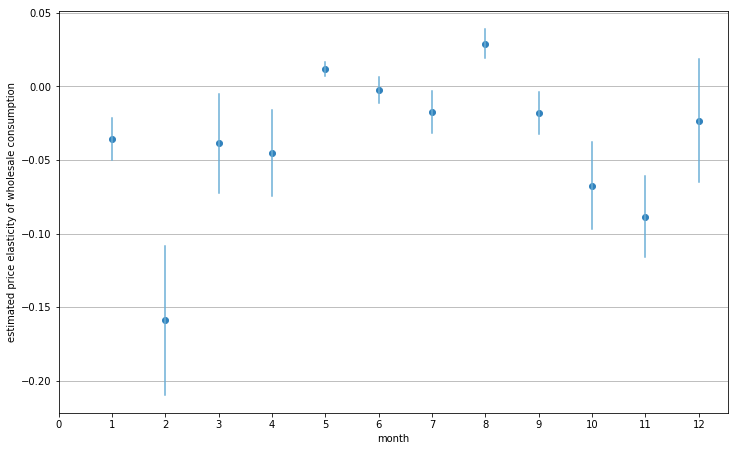
\includegraphics[width=1 \textwidth]{03_figures/ws_elasticity_month}
\end{figure}


\begin{landscape}
\begin{table}[H]
\centering
\begin{threeparttable}
  \caption{log wholesale electricity consumption by large grid areas, business days, hours 11-15 (P2SLS)}
  \label{tab:ws_grids_large}
  \footnotesize
    \begin{tabular}{lccccc}\toprule
                    &(1) N1 (DK1)   &(2) Konstant (DK1)   &(3) Evonet (DK1)   &(4) Cerius (DK2)   &(5) Radius (DK2)   \\
                    &        b/se   &        b/se   &        b/se   &        b/se   &        b/se   \\
\midrule
log spot price      &     -0.0347***&     -0.0082** &     -0.0569***&      0.0168***&     -0.0114***\\
                    &    (0.0051)   &    (0.0033)   &    (0.0051)   &    (0.0062)   &    (0.0028)   \\
log wholesale meters&      0.5122***&      0.7768***&      3.0910***&      0.2486***&     -0.2962***\\
                    &    (0.0894)   &    (0.0399)   &    (0.5103)   &    (0.0786)   &    (0.0423)   \\
Temperature         &     -0.0043***&     -0.0023***&     -0.0043***&     -0.0017***&     -0.0044***\\
                    &    (0.0005)   &    (0.0003)   &    (0.0005)   &    (0.0005)   &    (0.0003)   \\
Temperature squared &      0.0002***&      0.0001***&      0.0002***&      0.0001***&      0.0002***\\
                    &    (0.0000)   &    (0.0000)   &    (0.0000)   &    (0.0000)   &    (0.0000)   \\
Time variables      &         Yes   &         Yes   &         Yes   &         Yes   &         Yes   \\
\midrule
Adj. \(R^2\)        &      0.8649   &      0.8125   &      0.8062   &      0.6474   &      0.8613   \\
Observations        &       3,675   &       3,675   &       3,675   &       3,675   &       3,675   \\
\bottomrule\end{tabular}

    \begin{tablenotes}
    \item Robust standard errors are in parentheses below each estimate. * p<0.10, ** p<0.05, *** p<0.01.
    \item Log spot price is instrumented for by wind power prognosis for the same region.
  \end{tablenotes}
\end{threeparttable}
\end{table}

\end{landscape}
